\documentclass[11pt]{article}
\usepackage{graphicx} % Required for inserting images
\usepackage{tabularx}
\usepackage{algorithm}
\usepackage{changepage}
\usepackage{amsmath}
\usepackage{enumitem}
\usepackage{pgfplots}
\usepackage{algpseudocode}
\usepackage[a4paper,
            left=0.6in,
            top=1.0in,
            right=0.6in]{geometry}

\title{Networked software for distributed systems\\Project 5}
\date{2022-2023}

\begin{document}

\begin{titlepage}
\begin{center}
		\begin{figure}[ht]
			\centering
\includegraphics[width=0.7\textwidth]{resources/Logo_Politecnico_Milano.png}
		\end{figure}
        
        \vspace{3.5cm}

        \LARGE
        \textit{Networked software for distributed systems}\\

        \vspace{0.5cm}
        \Large
        \textbf{Analysis of COVID-19 Data}
        
        \vspace{\fill}
  
		\large
		\begin{tabularx}{\linewidth}{@{}lXl@{}}
			\textit{Authors:}  & & \textit{Professors:} \\
			Stefano Carraro      & & Prof.\@ Luca Mottola\\
			Stefano Fossati  & & Prof. Alessandro Margara \\
			Andrea Restelli & & \\
		\end{tabularx}		
		\thispagestyle{empty}

        \vspace{1cm}

        2022-2023
           
\end{center}
\end{titlepage}

\tableofcontents
\cleardoublepage

%%%
\section{Introduction}
\subsection{Request}
\subsubsection{Description}
Scientists increasingly use computer simulations to study complex phenomena. In this project, you have to implement a program that simulates how a virus spreads over time in a population of individuals. The program considers N individuals that move in a rectangular area with linear motion and velocity v (each individual following a different direction). Some individuals are initially infected. If an individual remains close to (at least one) infected individual for more than 10 minutes, it becomes infected. After 10 days, an infected individual recovers and becomes immune. Immune individuals do not become infected and do not infect others. An immune individual becomes susceptible again (i.e., it can be infected) after 3 months.
The overall area is split into smaller rectangular sub-areas representing countries. The program outputs, at the end of each simulated day, the overall number of susceptible, infected, and immune individuals in each country. An individual belongs to a country if it is in that country at the end of the day.
A performance analysis of the proposed solution is appreciated (but not mandatory). In particular, we are interested in studies that evaluate (1) how the execution time changes when increasing the number of individuals and/or the number of countries in the simulation; (2) how the execution time decreases when adding more processing cores/hosts. 
\subsubsection{Assumption and Guidelines}
\begin{itemize}
    \item The program takes in input the following parameters
    \begin{itemize}
        \item N = number of individuals
        \item I = number of individuals that are initially infected
        \item W, L = width and length of the rectangular area where individuals move (in meters)
        \item w, l = width and length of each country (in meters)
        \item v = moving speed for an individual
        \item d = maximum spreading distance (in meters): a susceptible individual that remains closer than d to at least one infected individual becomes infected 
        \item t = time step (in seconds): the simulation recomputes the position and status (susceptible, infected, immune) of each individual with a temporal granularity of t (simulated) seconds
    \end{itemize}
    \item You can make any assumptions on the behavior of individuals when they reach the boundaries of the area (for instance, they can change direction to guarantee that they remain in the area)
\end{itemize}
\subsubsection{Technologies}
Since the project involves a computationally heavy simulation that are suitable for parallel processing, we have chosen to use MPI (Message Passing Interface) as our parallel computing platform. MPI provides a standard for parallel computation and is well-suited for our simulation's computational requirements.

%%%%

%\cleardoublepage

\section{Project analysis and considerations}
\subsection{Considerations}
Initially, we explored two different approaches and thoroughly evaluated the optimal design choice. The first approach involved evenly distributing the population among processes, while the second approach divided the entire area into subareas and assigned each subarea to a process.

After careful consideration, we analyzed the advantages and disadvantages of each design proposal:
\begin{itemize}
    \item First approach:
    \begin{itemize}
        \item \textit{Advantages}: This design ensured an equal distribution of computation among processes, especially for updating the population's positions.
        \item \textit{Disadvantages}: Each process needed to be aware of the location of all infected individuals to perform infection checks. This approach required significant communication overhead and raised concerns about the computational complexity of infection control.
    \end{itemize}
    \item Second approach:
    \begin{itemize}
        \item \textit{Advantages}: With this design, each process only managed a specific portion of the population in a particular subarea. Consequently, the communication requirement was reduced to sending information about individuals moving between areas.
        \item \textit{Disadvantages}: In the worst-case scenario, where all individuals were concentrated in a single subarea managed by a single process, potential bottlenecks could arise. Additionally, managing infections became more complex when non-infected and infected individuals were located in different process areas but in close proximity on the borders.
    \end{itemize}
\end{itemize}

After careful consideration, we chose the first approach to minimize assumptions and ensure an evenly distributed workload among processes. However, it's important to note that the network could potentially become a bottleneck in this approach.

\subsection{Additional Assumptions}
\begin{itemize}
    \item Individuals move in a random direction every time their position is updated.
    \item Individuals reappear in the other side of the area, so specularly to the center of the rectangle,  if they overcome the boundaries of the whole area.
    \item Non-infected individuals become infected if and only if they are near at least one infected person for 10 consecutive minutes.
    \item Parameters W, L are multiple of w, l.
    \item Number of individuals \(\gg\) number of countries.
\end{itemize}


\section{Design and Implementation}
In this section, we provide a brief overview of how our simulation algorithm works. Additionally, at the end of the section we present the detailed pseudocode of the algorithm.
\subsection{World and countries organization}
As the world of our simulation, we consider a rectangular area of dimensions \(W \times L\), where each country has dimensions \(w \times l\). The countries are organized in a grid structure, as illustrated in Figure \ref{fig:world}. In the figure, the indexing criteria for the countries are also shown, indicating the row and column indices of each country.
\begin{figure}[h]
    \centering
    \label{fig:world}
    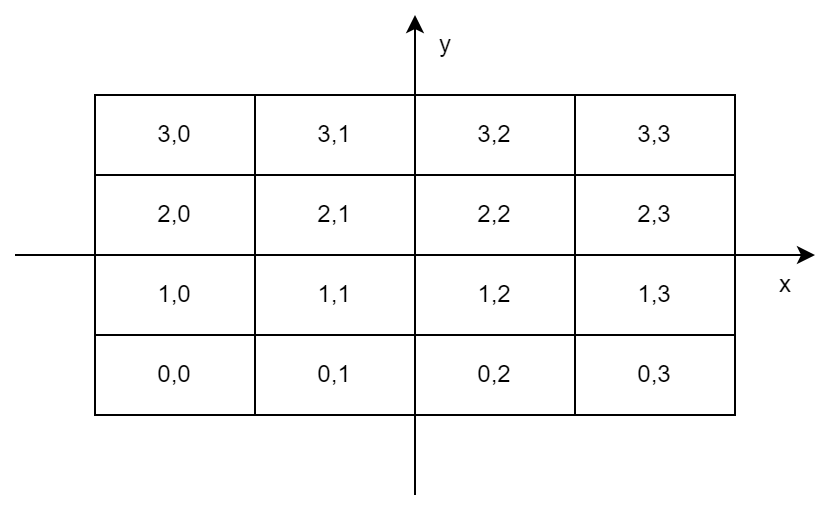
\includegraphics[width=0.4\textwidth]{resources/world.png}
    \caption{World and countries distribution}
\end{figure}
\subsection{Algorithm implementation}
The simulation algorithm is divided into three main phases.
\begin{enumerate}[label=\textbf{\arabic*.}, leftmargin=*]
        \item \textbf{Input reading.} In this phase, the leader process reads the simulation parameters from a configuration file. After performing a validity check on the parameters, the leader distributes them to all other processes using a \texttt{Bcast} operation. Although a \texttt{Scatter} operation could have been used since the data to be sent are primitive integers, we chose broadcasting the configuration struct to minimize communication traffic. 
    \item \textbf{Simulation step.} This is the central phase of the algorithm, where each process performs the following steps: 
    \begin{itemize}
        \item Update the position of the individuals it manages.
        \item Send the list of infected individuals to the leader.
        \item Receive the list of all infected individuals from the leader.
        \item Update the status of each individual it manages.
    \end{itemize}
    \item \textbf{Report building.} At the end of each day (i.e. when t is a multiple of 86400 seconds), each process sends an array to the leader. The array contains, for each country, the counts of NON\_INFECTED, INFECTED and IMMUNE individuals among those it manages. The leader collects all the received reports, merges them, and creates a consolidated daily case report for the day. The report is then written to a CSV file.
\end{enumerate}
Figure \ref{fig:flow} illustrates the three phases described above in a visual diagram to facilitate comprehension.

\begin{figure}[h]
    \centering
    \label{fig:flow}
    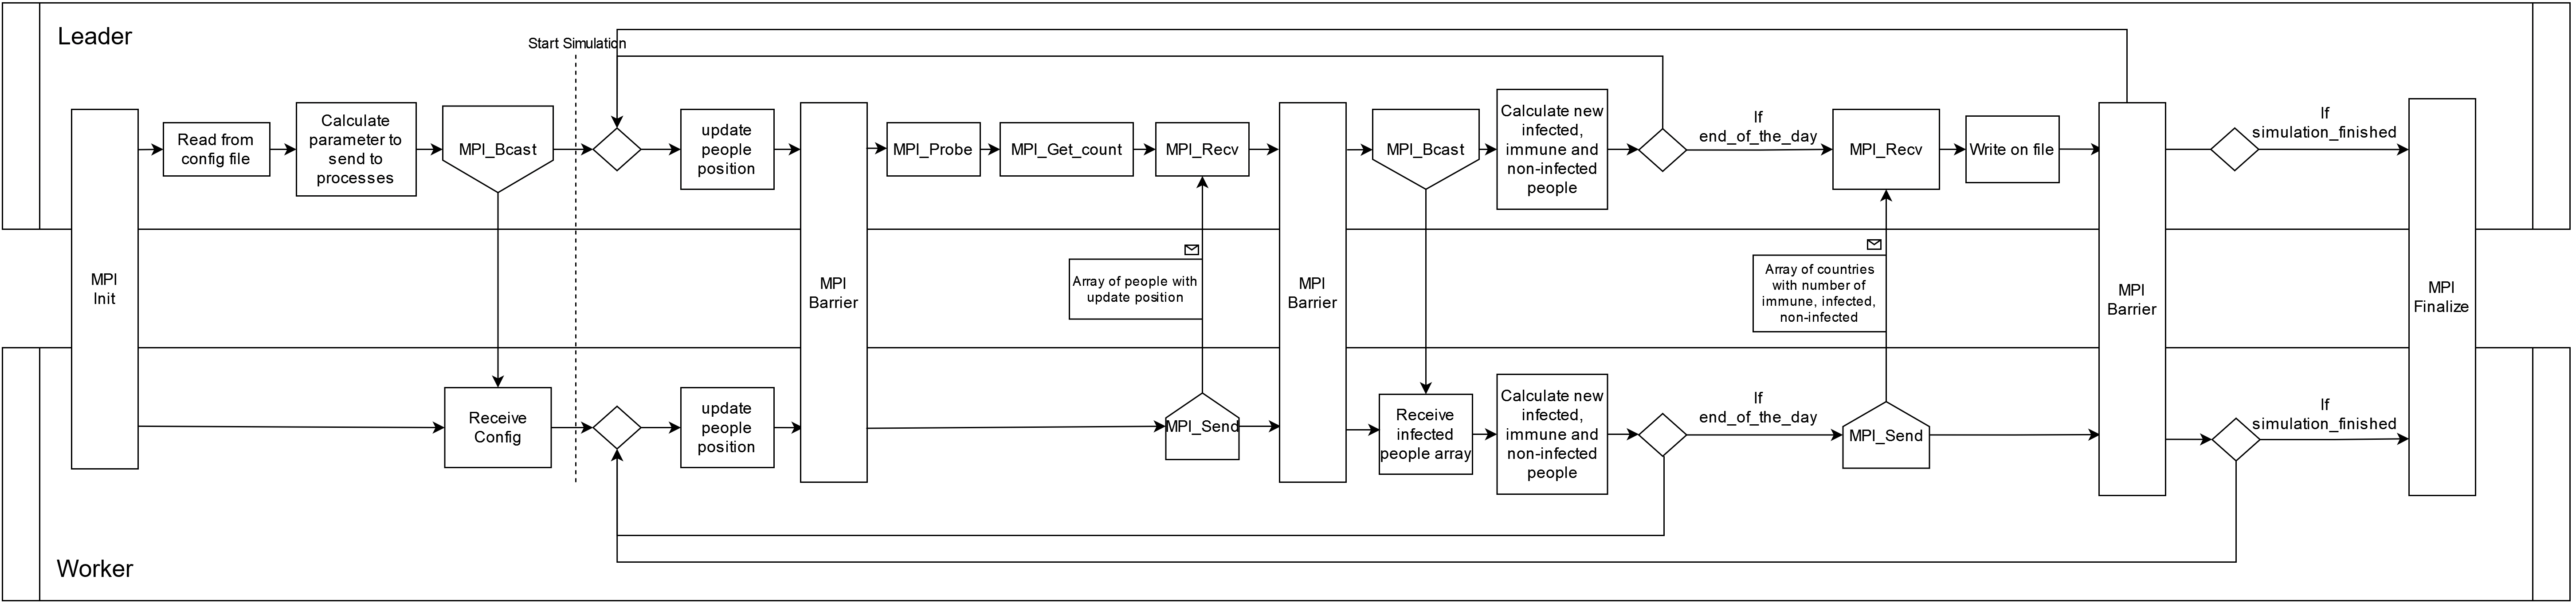
\includegraphics[width=1\textwidth]{resources/MPI_flow.png}
    \caption{MPI processes call schema}
\end{figure}
\begin{algorithm}[H]
\caption{Simulation Algorithm}\label{alg:cap}
    \begin{algorithmic}
        \If{is Leader}
            \State Leader reads from file the simulation parameters
            \State Leader calculates the number of countries, how many non-infected and infected  individuals for each process 
        \EndIf
        \State Broadcast of the simulation parameters (MPI\_Broad)
        \While{$time < total time$}
            \State compute the new position
            \If{is not Leader} 
                \State Send infected individuals to the leader (MPI\_Send)
            \ElsIf{is Leader}
                \State Receive infected individuals from non-leader processes (MPI\_Recv)
            \EndIf
            \If{is Leader} 
                \State Broadcast infected\_individuals
            \EndIf
            \For{$each$ individual}
				\If{IMMUNE $||$ INFECTED}
                    \State decrease timer
                \ElsIf{NON-INFECTED}
                    \For{$each$ infected\_individual}
                        \If{NON-INFECTED is near INFECTED}
                            \State Decrease timer
                        \ElsIf{}
                            \State Reset timer
                        \EndIf
                    \EndFor
                \EndIf
			\EndFor

            \If{is end of the day}
                \State Compute how many non-infected, infected and immune in each country
                \If{is not leader}
                    \State Send information to the leader (MPI\_Send)
                \ElsIf{leader}
                    \State Receive information from all non leader processes (MPI\_Recv)
                    \State Merge the data
                    \State Write the data on file
                \EndIf
            \EndIf
        \EndWhile
        
    \end{algorithmic}
\end{algorithm}
\section{Performance Analysis}
In this section we analyze how the \textit{execution time} evolves by varying the number of individuals \textit{I} and the number of countries \textit{C}, as well as by adding more processing cores/hosts.

By analyzing the computational complexity of the designed algorithm we can make a theoretical forecast of the performance of the algorithm. We consider the following variables: 
\begin{itemize}
    \item \textit{N}, the number of individuals.
    \item \textit{W}, the number of worker processes.
    \item \(S = \left\lfloor \frac{{t_{\text{{total}}}}}{{t_{\text{{step}}}}} \right\rfloor\), the number of steps of the simulation.
\end{itemize}
We can easily see that the complexity is upper bounded by the loop, performed by each worker, going through each NON\_INFECTED individual and checking whether it is near at least one INFECTED individual. 

As a result the computational complexity of the algorithm is \[O\left(S \frac{N^2}{W}\right)\]

In the following subsections we explain the experiments we conducted to study the execution time variation when varying the variables affecting performances. For subsections \ref{subsec:individuals} and \ref{subsec:countries} we used 2 processing hosts with 6 cores each. For all the experiments, \(t_{\text{total}}\) was equal to \(30 \times 10^6\) seconds, more or less 347 days; \(t_{\text{step}}\) was equal to 5 minutes.



\subsection{Varying the number of individuals}
\label{subsec:individuals}
Our algorithm should be quite resilient to the growth in the number of individuals. This because, as previously highlighted, one of the advantages of our approach is to have an equal division among the working processes of the individuals to consider in the simulation. 
\begin{figure}[h]
\caption{Varying the number of individuals}
\begin{minipage}{0.5\textwidth}
  \centering
  \begin{tabular}{|c|c|}
    \hline
    \textbf{N} & \textbf{Execution Time} \\
    \hline
    10000 & 144s \\ 
    15000 & 166s \\ 
    20000 & 163s \\ 
    25000 & 173s \\
    30000 & 181s \\
    40000 & 203s \\
    50000 &  227s \\
    60000 & 294s \\
    \hline
  \end{tabular}
\end{minipage}%
\centering
\begin{minipage}{0.5\textwidth}
      \label{fig:individuals}
      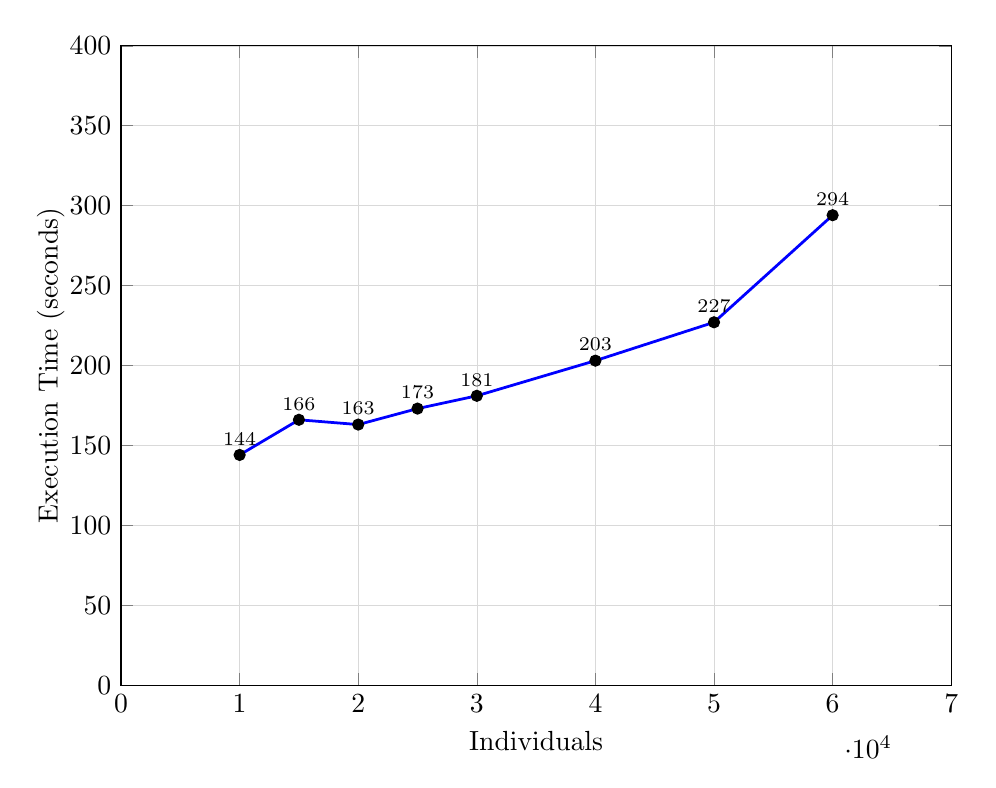
\begin{tikzpicture}
        \begin{axis}[
            xlabel={Individuals},
            ylabel={Execution Time (seconds)},
            xmin=0, xmax=70000,
            ymin=0, ymax=400,
            grid=both,
            grid style={line width=0.2pt, draw=gray!30},
            width=\textwidth,
            height=0.8\textwidth,
            mark=none,
            ylabel style={yshift=-5pt}
          ]
          \addplot[
            scatter,
            only marks,
            mark=*,
            nodes near coords,
            point meta=explicit symbolic,
            every node near coord/.append style={anchor=south, font=\scriptsize},
          ] table[meta index=2] {
          x     y     label
          10000   144   144
          15000   166   166
          20000   163   163
          25000   173   173
          30000   181   181
          40000   203   203
          50000   227  227
          60000   294  294
        };
        \addplot[
            line width=1pt,
            color=blue,
            mark=none,
          ] table {
          x     y
          10000   144
          15000   166
          20000   163
          25000   173
          30000   181
          40000   203
          50000   227
          60000   294
        };
      \end{axis}
      \end{tikzpicture}
    \end{minipage}
\end{figure}

The main challenge in this case was to find an optimal equilibrium between parameters in order to avoid an early termination of the simulation due to lack of infectable individuals.
However, the results obtained are more or less in line with what we expected: increasing the number of individuals doesn't make the curve of the execution time to explode exponentially.

\subsection{Varying the number of countries}
\label{subsec:countries}
Our algorithm is designed to be unaffected by variations in the number of countries. This is because we only consider them at the end of the day when computing the daily report of cases. We merge the reports obtained by worker processes for the individuals they manage. We would also expect a slight decrease in performance as the number of countries increases since more reports need to be merged. As expected, the execution time of our algorithm remains stable and unaffected by the number of countries, as shown in Figure \ref{fig:countries}.

\begin{figure}[h]
\caption{Varying the number of countries}
\label{fig:countries}
\vspace{4pt}
\begin{minipage}{0.5\textwidth}
  \centering
  \begin{tabular}{|c|c|}
    \hline
    \textbf{C} & \textbf{Execution Time} \\
    \hline
    1 &  185s\\ 
    4 &  189s\\ 
    16 &  192s\\ 
    64 &  186s\\
    128 & 193s\\
    \hline
  \end{tabular}
\end{minipage}%
\centering
\begin{minipage}{0.5\textwidth}
      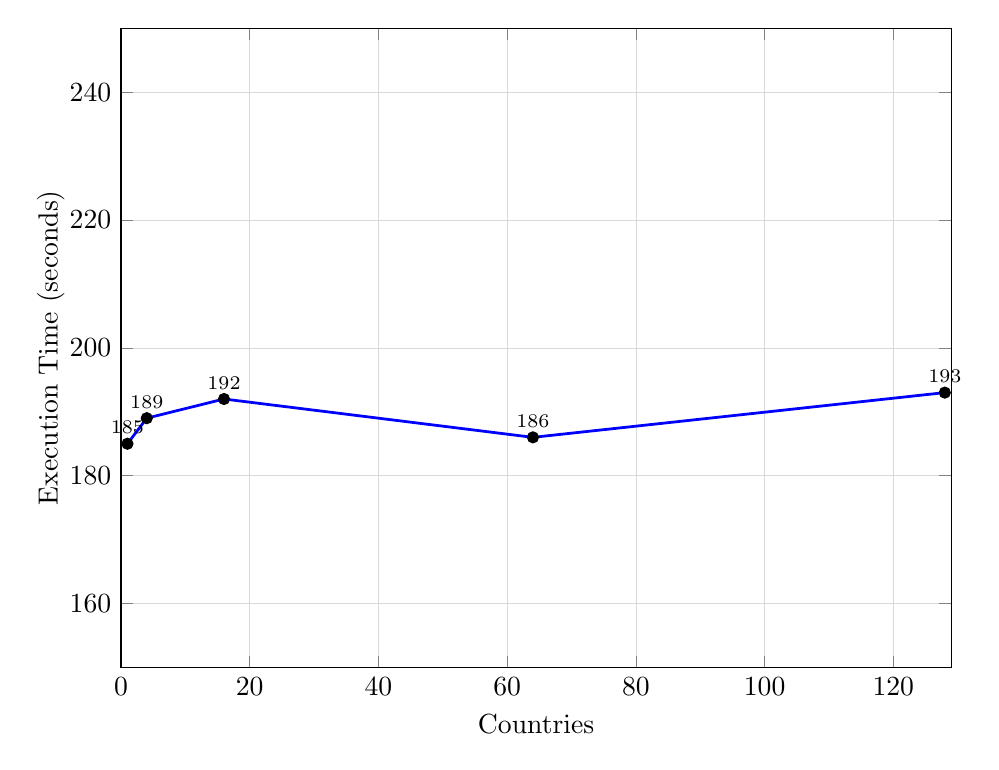
\begin{tikzpicture}
        \begin{axis}[
            xlabel={Countries},
            ylabel={Execution Time (seconds)},
            xmin=0, xmax=129,
            ymin=150, ymax=250,
            grid=both,
            grid style={line width=0.2pt, draw=gray!30},
            width=\textwidth,
            height=0.8\textwidth,
            mark=none,
            ylabel style={yshift=-5pt}
          ]
          \addplot[
            scatter,
            only marks,
            mark=*,
            nodes near coords,
            point meta=explicit symbolic,
            every node near coord/.append style={anchor=south, font=\scriptsize},
          ] table[meta index=2] {
          x     y     label
          1    185   185 
          4    189   189
          16   192   192
          64   186   186
          128  193   193
        };
        \addplot[
            line width=1pt,
            color=blue,
            mark=none,
          ] table {
          x     y
          1    185
          4    189
          16   192
          64   186
          128  193
        };
      \end{axis}
      \end{tikzpicture}
    \end{minipage}
\end{figure}

\subsection{Adding more hosts}
\label{subsec:hosts}
As highlighted in the computational complexity analysis of our algorithm, the performance is expected to improve with the addition of more hosts and processes. This expectation is confirmed by our experiment, where we considered 4 hosts, each with 2 cores (with the number of available cores limited to the minimum among them to ensure a fair comparison). We incrementally added hosts to the computation and observed the corresponding execution times.

From Figure \ref{fig:hosts}, we can observe that, as anticipated, the execution time decreases as we add more hosts. However, an interesting observation is that when transitioning from 3 to 4 hosts, the performance actually decreases. We attribute this decrease to the fact that the advantage gained by adding 2 more cores to the computation is not sufficient to compensate for the decrease in performance caused by the latency introduced by the increased communication overhead among hosts.

\begin{figure}[h]
\caption{Varying the number of hosts}
\label{fig:hosts}
\begin{minipage}{0.5\textwidth}
  \centering
  \begin{tabular}{|c|c|}
    \hline
    \textbf{I} & \textbf{Execution Time} \\
    \hline
    1 & 407s \\ 
    2 & 271s \\ 
    3 & 211s \\ 
    4 & 234s \\
    \hline
  \end{tabular}
\end{minipage}%
\centering
\begin{minipage}{0.5\textwidth}
      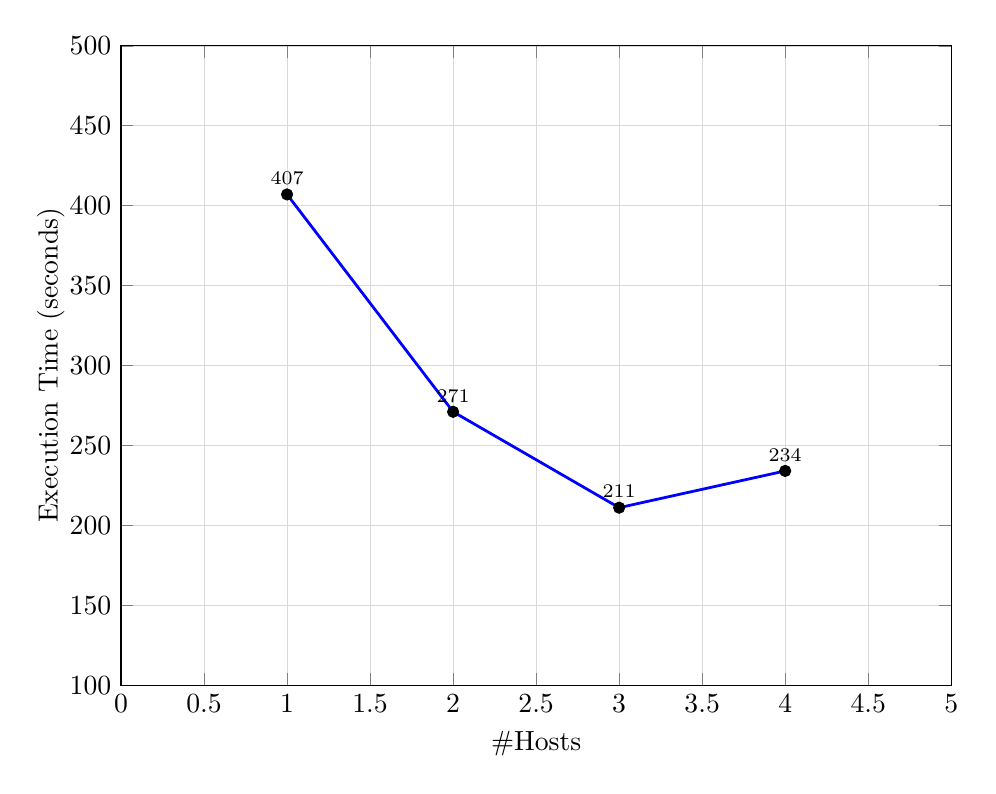
\begin{tikzpicture}
        \begin{axis}[
            xlabel={\#Hosts},
            ylabel={Execution Time (seconds)},
            xmin=0, xmax=5,
            ymin=100, ymax=500,
            grid=both,
            grid style={line width=0.2pt, draw=gray!30},
            width=\textwidth,
            height=0.8\textwidth,
            mark=none,
            ylabel style={yshift=-5pt}
          ]
          \addplot[
            scatter,
            only marks,
            mark=*,
            nodes near coords,
            point meta=explicit symbolic,
            every node near coord/.append style={anchor=south, font=\scriptsize},
          ] table[meta index=2] {
          x     y     label
          1    407   407 
          2   271   271
          3   211   211
          4   234   234
        };
        \addplot[
            line width=1pt,
            color=blue,
            mark=none,
          ] table {
          x     y
          1    407
          2    271
          3    211
          4    234
        };
      \end{axis}
    \end{tikzpicture}
    \end{minipage}
\end{figure}

\end{document}
